Encuentra el valor de $x$ en el siguiente triángulo isóceles:

% \begin{minipage}[t][][t]{0.3\textwidth}
\begin{figure}[H]
    \centering
    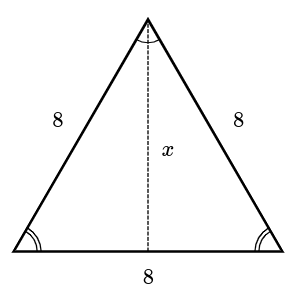
\includegraphics[width=0.2\linewidth]{../images/pitagoras12.png}
    \caption{}
    \label{fig:pitagoras12}
\end{figure}
% \end{minipage}\hfill
% \begin{minipage}[t][][t]{0.68\textwidth}
\begin{solutionbox}{15cm}
    \begin{minipage}{0.3\textwidth}
        \begin{figure}[H]
            \centering
            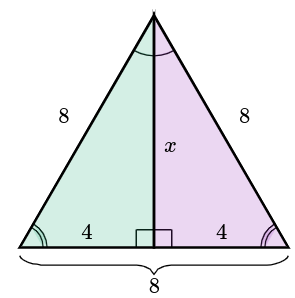
\includegraphics[width=0.6\linewidth]{../images/pitagoras12a.png}
            \caption{}
            \label{fig:pitagoras12a}
        \end{figure}
        \begin{figure}[H]
            \centering
            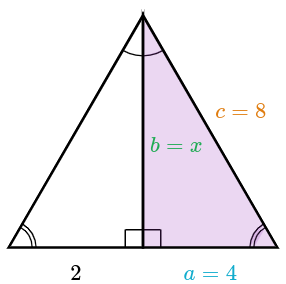
\includegraphics[width=0.6\linewidth]{../images/pitagoras12b.png}
            \caption{}
            \label{fig:pitagoras12b}
        \end{figure}
    \end{minipage}\hfill
    \begin{minipage}{0.65\textwidth}
        Podemos utilizar el teorema de Pitágoras para encontrar un lado faltante.
        La ecuación del teorema de Pitágoras es:
        \[c^2=a^2+b^2\]
        donde $a$ y $b$ son las longitudes de los catetos, y $c$ es la longitud de la hipotenusa.
        En este caso, $a=83$, $b=x$ y $c=158$, Entonces,
        \begin{align*}
            83^2+x^2  & =158^2         \\
            6,889+x^2 & =24,964        \\
            x^2       & =18,075        \\
            x^2       & =\sqrt{18,075} \\
            x         & \sim 134.443
        \end{align*}
        El extremo de la rampa estará a $134.4$ centímetros de la parte trasera del camión.
    \end{minipage}
\end{solutionbox}
% \end{minipage}
